\tikzset{every picture/.style={line width=0.75pt}} %set default line width to 0.75pt        

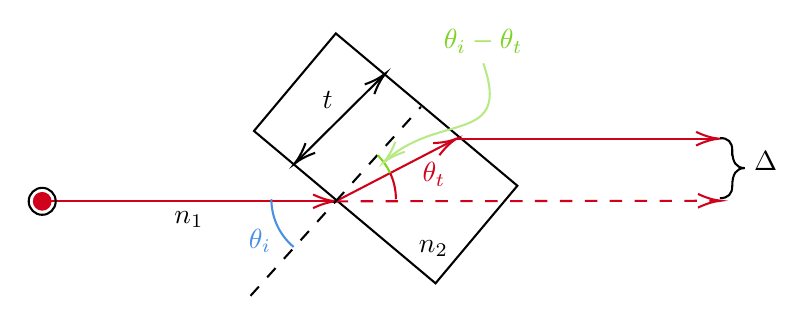
\begin{tikzpicture}[x=0.75pt,y=0.75pt,yscale=-1,xscale=1]
%uncomment if require: \path (0,444); %set diagram left start at 0, and has height of 444

%Straight Lines [id:da3089462694390681] 
\draw [color={rgb, 255:red, 208; green, 2; blue, 27 }  ,draw opacity=1 ]   (106.5,135.5) -- (245.92,135.5) ;
\draw [shift={(247.92,135.5)}, rotate = 180] [color={rgb, 255:red, 208; green, 2; blue, 27 }  ,draw opacity=1 ][line width=0.75]    (10.93,-3.29) .. controls (6.95,-1.4) and (3.31,-0.3) .. (0,0) .. controls (3.31,0.3) and (6.95,1.4) .. (10.93,3.29)   ;
%Shape: Circle [id:dp687997837864077] 
\draw   (100,135.5) .. controls (100,131.91) and (102.91,129) .. (106.5,129) .. controls (110.09,129) and (113,131.91) .. (113,135.5) .. controls (113,139.09) and (110.09,142) .. (106.5,142) .. controls (102.91,142) and (100,139.09) .. (100,135.5) -- cycle ;
%Shape: Circle [id:dp6466863455580079] 
\draw  [color={rgb, 255:red, 208; green, 2; blue, 27 }  ,draw opacity=1 ][fill={rgb, 255:red, 208; green, 2; blue, 27 }  ,fill opacity=1 ] (102.5,135.5) .. controls (102.5,133.29) and (104.29,131.5) .. (106.5,131.5) .. controls (108.71,131.5) and (110.5,133.29) .. (110.5,135.5) .. controls (110.5,137.71) and (108.71,139.5) .. (106.5,139.5) .. controls (104.29,139.5) and (102.5,137.71) .. (102.5,135.5) -- cycle ;
%Shape: Rectangle [id:dp5570623200210392] 
\draw   (247.97,54.61) -- (335.44,128) -- (296,175) -- (208.53,101.6) -- cycle ;
%Straight Lines [id:da14924518496374972] 
\draw [color={rgb, 255:red, 208; green, 2; blue, 27 }  ,draw opacity=1 ]   (247.92,135.5) -- (304.28,106.25) ;
\draw [shift={(306.05,105.33)}, rotate = 152.57] [color={rgb, 255:red, 208; green, 2; blue, 27 }  ,draw opacity=1 ][line width=0.75]    (10.93,-3.29) .. controls (6.95,-1.4) and (3.31,-0.3) .. (0,0) .. controls (3.31,0.3) and (6.95,1.4) .. (10.93,3.29)   ;
%Straight Lines [id:da36139448467369784] 
\draw [color={rgb, 255:red, 208; green, 2; blue, 27 }  ,draw opacity=1 ]   (306.05,105.33) -- (430.47,105.33) ;
\draw [shift={(432.47,105.33)}, rotate = 180] [color={rgb, 255:red, 208; green, 2; blue, 27 }  ,draw opacity=1 ][line width=0.75]    (10.93,-3.29) .. controls (6.95,-1.4) and (3.31,-0.3) .. (0,0) .. controls (3.31,0.3) and (6.95,1.4) .. (10.93,3.29)   ;
%Straight Lines [id:da36996139499499425] 
\draw [color={rgb, 255:red, 208; green, 2; blue, 27 }  ,draw opacity=1 ] [dash pattern={on 4.5pt off 4.5pt}]  (247.92,135.5) -- (431.4,135.23) ;
\draw [shift={(433.4,135.22)}, rotate = 179.91] [color={rgb, 255:red, 208; green, 2; blue, 27 }  ,draw opacity=1 ][line width=0.75]    (10.93,-3.29) .. controls (6.95,-1.4) and (3.31,-0.3) .. (0,0) .. controls (3.31,0.3) and (6.95,1.4) .. (10.93,3.29)   ;
%Shape: Brace [id:dp7371764969387753] 
\draw   (433,134) .. controls (436.98,134) and (438.97,132.01) .. (438.97,128.03) -- (438.97,128.03) .. controls (438.97,122.34) and (440.96,119.5) .. (444.94,119.5) .. controls (440.96,119.5) and (438.97,116.66) .. (438.97,110.97)(438.97,113.53) -- (438.97,110.97) .. controls (438.97,106.99) and (436.98,105) .. (433,105) ;
%Shape: Arc [id:dp6592082376861983] 
\draw  [draw opacity=0] (274.12,121.82) .. controls (275.92,125.67) and (276.92,129.97) .. (276.92,134.5) -- (246.92,134.5) -- cycle ; \draw  [color={rgb, 255:red, 208; green, 2; blue, 27 }  ,draw opacity=1 ] (274.12,121.82) .. controls (275.92,125.67) and (276.92,129.97) .. (276.92,134.5) ;  
%Straight Lines [id:da10825483880415332] 
\draw    (229.34,116.09) -- (270.56,75.21) ;
\draw [shift={(271.98,73.8)}, rotate = 135.24] [color={rgb, 255:red, 0; green, 0; blue, 0 }  ][line width=0.75]    (10.93,-3.29) .. controls (6.95,-1.4) and (3.31,-0.3) .. (0,0) .. controls (3.31,0.3) and (6.95,1.4) .. (10.93,3.29)   ;
\draw [shift={(227.92,117.5)}, rotate = 315.24] [color={rgb, 255:red, 0; green, 0; blue, 0 }  ][line width=0.75]    (10.93,-3.29) .. controls (6.95,-1.4) and (3.31,-0.3) .. (0,0) .. controls (3.31,0.3) and (6.95,1.4) .. (10.93,3.29)   ;
%Straight Lines [id:da5061477765805575] 
\draw  [dash pattern={on 4.5pt off 4.5pt}]  (247.92,135.5) -- (288.97,89.97) ;
%Shape: Arc [id:dp8090227623570767] 
\draw  [draw opacity=0] (268.13,113.29) .. controls (270.59,115.75) and (272.63,118.63) .. (274.12,121.82) -- (246.92,134.5) -- cycle ; \draw  [color={rgb, 255:red, 126; green, 211; blue, 33 }  ,draw opacity=1 ] (268.13,113.29) .. controls (270.59,115.75) and (272.63,118.63) .. (274.12,121.82) ;  
%Straight Lines [id:da6394647938540519] 
\draw  [dash pattern={on 4.5pt off 4.5pt}]  (206.87,181.03) -- (247.92,135.5) ;
%Shape: Arc [id:dp9776143180986732] 
\draw  [draw opacity=0] (227.64,157.48) .. controls (221.09,151.98) and (216.92,143.73) .. (216.92,134.5) .. controls (216.92,134.5) and (216.92,134.5) .. (216.92,134.5) -- (246.92,134.5) -- cycle ; \draw  [color={rgb, 255:red, 74; green, 144; blue, 226 }  ,draw opacity=1 ] (227.64,157.48) .. controls (221.09,151.98) and (216.92,143.73) .. (216.92,134.5) .. controls (216.92,134.5) and (216.92,134.5) .. (216.92,134.5) ;  
%Curve Lines [id:da00684858507634134] 
\draw [color={rgb, 255:red, 184; green, 233; blue, 134 }  ,draw opacity=1 ]   (319,69) .. controls (332.79,108.4) and (298.07,92.5) .. (272.16,115.71) ;
\draw [shift={(270.98,116.8)}, rotate = 316.37] [color={rgb, 255:red, 184; green, 233; blue, 134 }  ,draw opacity=1 ][line width=0.75]    (10.93,-3.29) .. controls (6.95,-1.4) and (3.31,-0.3) .. (0,0) .. controls (3.31,0.3) and (6.95,1.4) .. (10.93,3.29)   ;

% Text Node
\draw (448,116) node [anchor=west] [inner sep=0.75pt]    {$\Delta $};
% Text Node
\draw (177.21,138.9) node [anchor=north] [inner sep=0.75pt]    {$n_{1}$};
% Text Node
\draw (295,163.6) node [anchor=south] [inner sep=0.75pt]    {$n_{2}$};
% Text Node
\draw (247.95,92.25) node [anchor=south east] [inner sep=0.75pt]    {$t$};
% Text Node
\draw (218.23,147.4) node [anchor=north east] [inner sep=0.75pt]  [color={rgb, 255:red, 74; green, 144; blue, 226 }  ,opacity=1 ]  {$\theta _{i}$};
% Text Node
\draw (302.23,115.4) node [anchor=north east] [inner sep=0.75pt]  [color={rgb, 255:red, 208; green, 2; blue, 27 }  ,opacity=1 ]  {$\theta _{t}$};
% Text Node
\draw (319,65.6) node [anchor=south] [inner sep=0.75pt]  [color={rgb, 255:red, 126; green, 211; blue, 33 }  ,opacity=1 ]  {$\theta _{i} -\theta _{t}$};


\end{tikzpicture}
